\providecommand\ExamFontPath{../../../字体/}
\documentclass[fontset=exam]{exam-zh}
\usepackage{longtable,booktabs,array,calc,multirow,fvextra}
\usepackage[normalem]{ulem}
\providecommand{\hl}[1]{#1}
\providecommand{\ul}[1]{\uline{#1}}
\DefineVerbatimEnvironment{verbatim}{Verbatim}{breaklines=true,fontsize=\small}
\providecommand{\tightlist}{\setlength{\itemsep}{0pt}\setlength{\parskip}{0pt}}
\newcommand{\pandocbounded}[1]{#1}
\setlength{\emergencystretch}{3em}
\setlength{\tabcolsep}{2pt}
\examsetup{page/size=a4paper}
\title{厦门大学 2010 级期末试卷}
\subject[4em]{力学}
\begin{document}
\maketitle
\fancyfoot[C]{第 \thepage 页（共 \pageref*{LastPage} 页）}
\pdfbookmark[1]{一． 判断题（每小题2分，共20分。正确的在相应序号后打“√”，错误的打“×”。要求将答案写在答题纸上）}{section1}

一． 判断题（每小题 2 分，共 20 分。正确的在相应序号后打``√''，错误的打``×''。要求将答案写在答题纸上）

\begin{enumerate}
\def\labelenumi{\arabic{enumi}.}
\item
  当刚体作纯滚动时，作用在刚体上的静摩擦力总是与质心的运动方向相反。
\item
  刚体的质量越大，其转动惯量就越大，因而其转动惯性也越大。
\item
  刚体绕定轴转动时，其转动动能的增量等于刚体所受外力矩做功的代数和。
\item
  两同方向但不同频率的简谐振动合成后仍然为简谐振动。
\item
  一波源产生的平面简谐横波一段时间后将振动传播至某质点，该质点初始振动方向取决于它离波源的位置。
\item
  将弹簧振子的弹簧剪掉一半，其振动频率变为原来的 2 倍。
\item
  波源的振动速度越大，波传播的速度就越大。
\item
  在所有的惯性系中，真空光速具有相同量值，与光源的运动无关
\end{enumerate}

10.高速运动电子的质量随其运动速率的增大而增大

\pdfbookmark[1]{二．如图所示，质量为m_1，长为l的均匀细棒静止于水平桌面上。细棒可绕通过其端点O的竖直固定光滑轴转动。棒与桌面间的滑动}{section4}

二．如图所示，质量为\(m_{1}\)，长为\(l\)的均匀细棒静止于水平桌面上。细棒可绕通过其端点 O 的竖直固定光滑轴转动。棒与桌面间的滑动摩擦因为为\(\mu\)。今有一质量为\(m_{2}\)的滑块在水平面内以垂直于棒长方向的速度\(v_{1}\)与棒的下端相碰，碰撞后滑块的速度变为\(v_{\text{2}}\)，方向与\(v_{1}\)相反。试求：\par\medskip{\centering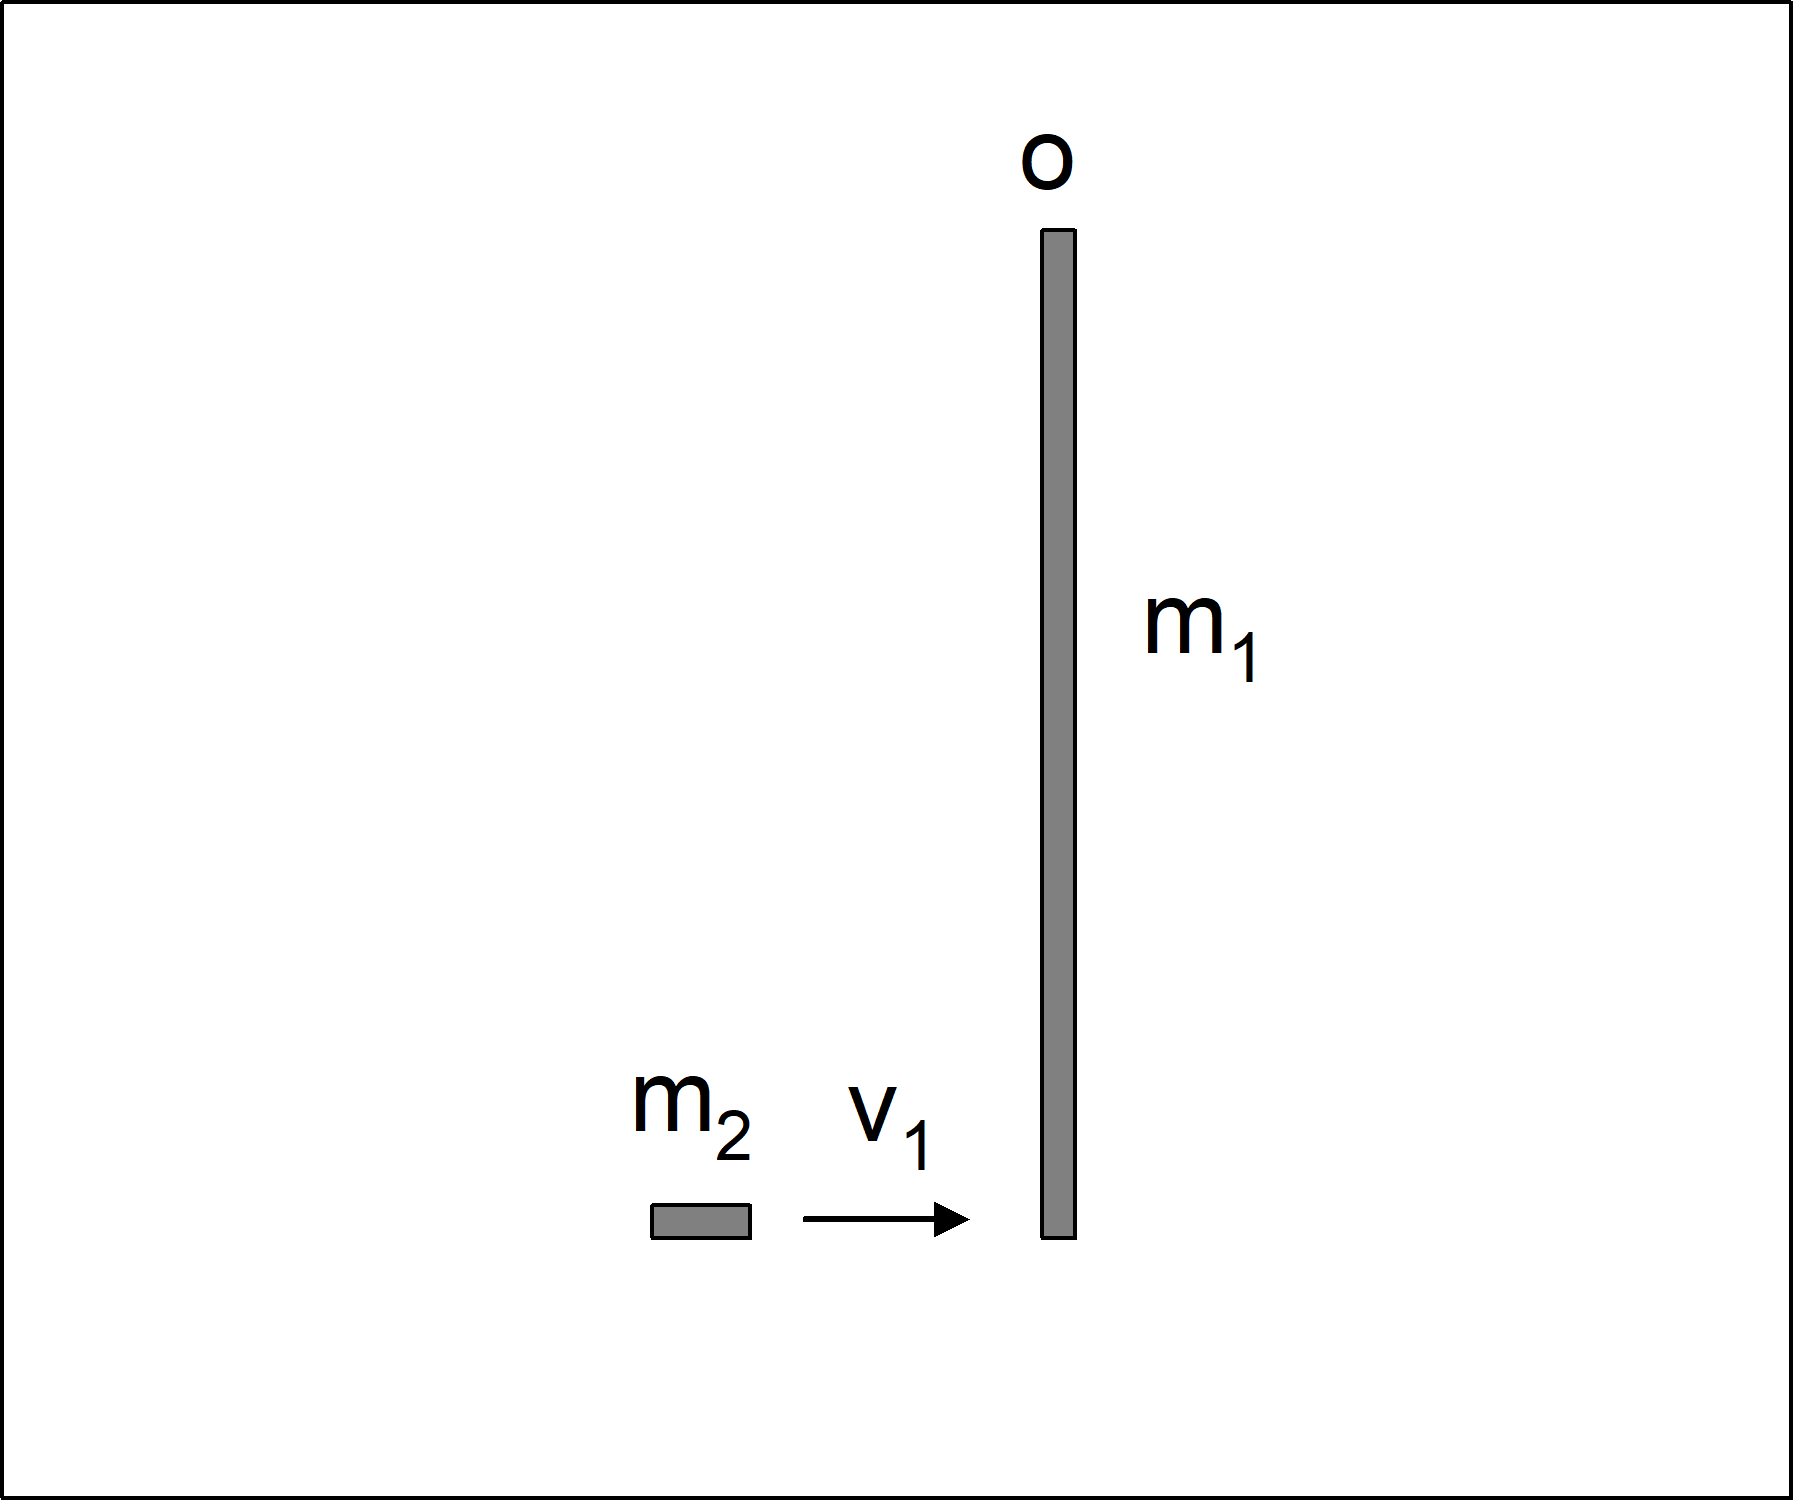
\includegraphics[width=5cm,height=4cm,keepaspectratio]{figures/image2.png}\par}\medskip

（1）滑块碰撞后棒所获得的角速度;

(2) 碰撞后棒在转动过程中所受的摩擦力矩;

(3) 碰撞后，从细棒开始转动到转动停止所经历的时间。

\pdfbookmark[1]{三． (16分) 如图，水平桌面上的均质圆柱体A上绕着轻绳，绳子跨过一定滑轮B后与物体C相连。设A、B、C的质量均为为m}{section8}

三． (16 分) 如图，水平桌面上的均质圆柱体 A 上绕着轻绳，绳子跨过一定滑轮 B 后与物体 C 相连。设 A、B、C 的质量均为为 m，圆柱体和定滑轮的半径均为 R，现系统从静止开始运动。若圆柱体与各接触点、定滑轮与绳子间都无相对滑动，试求\par\medskip{\centering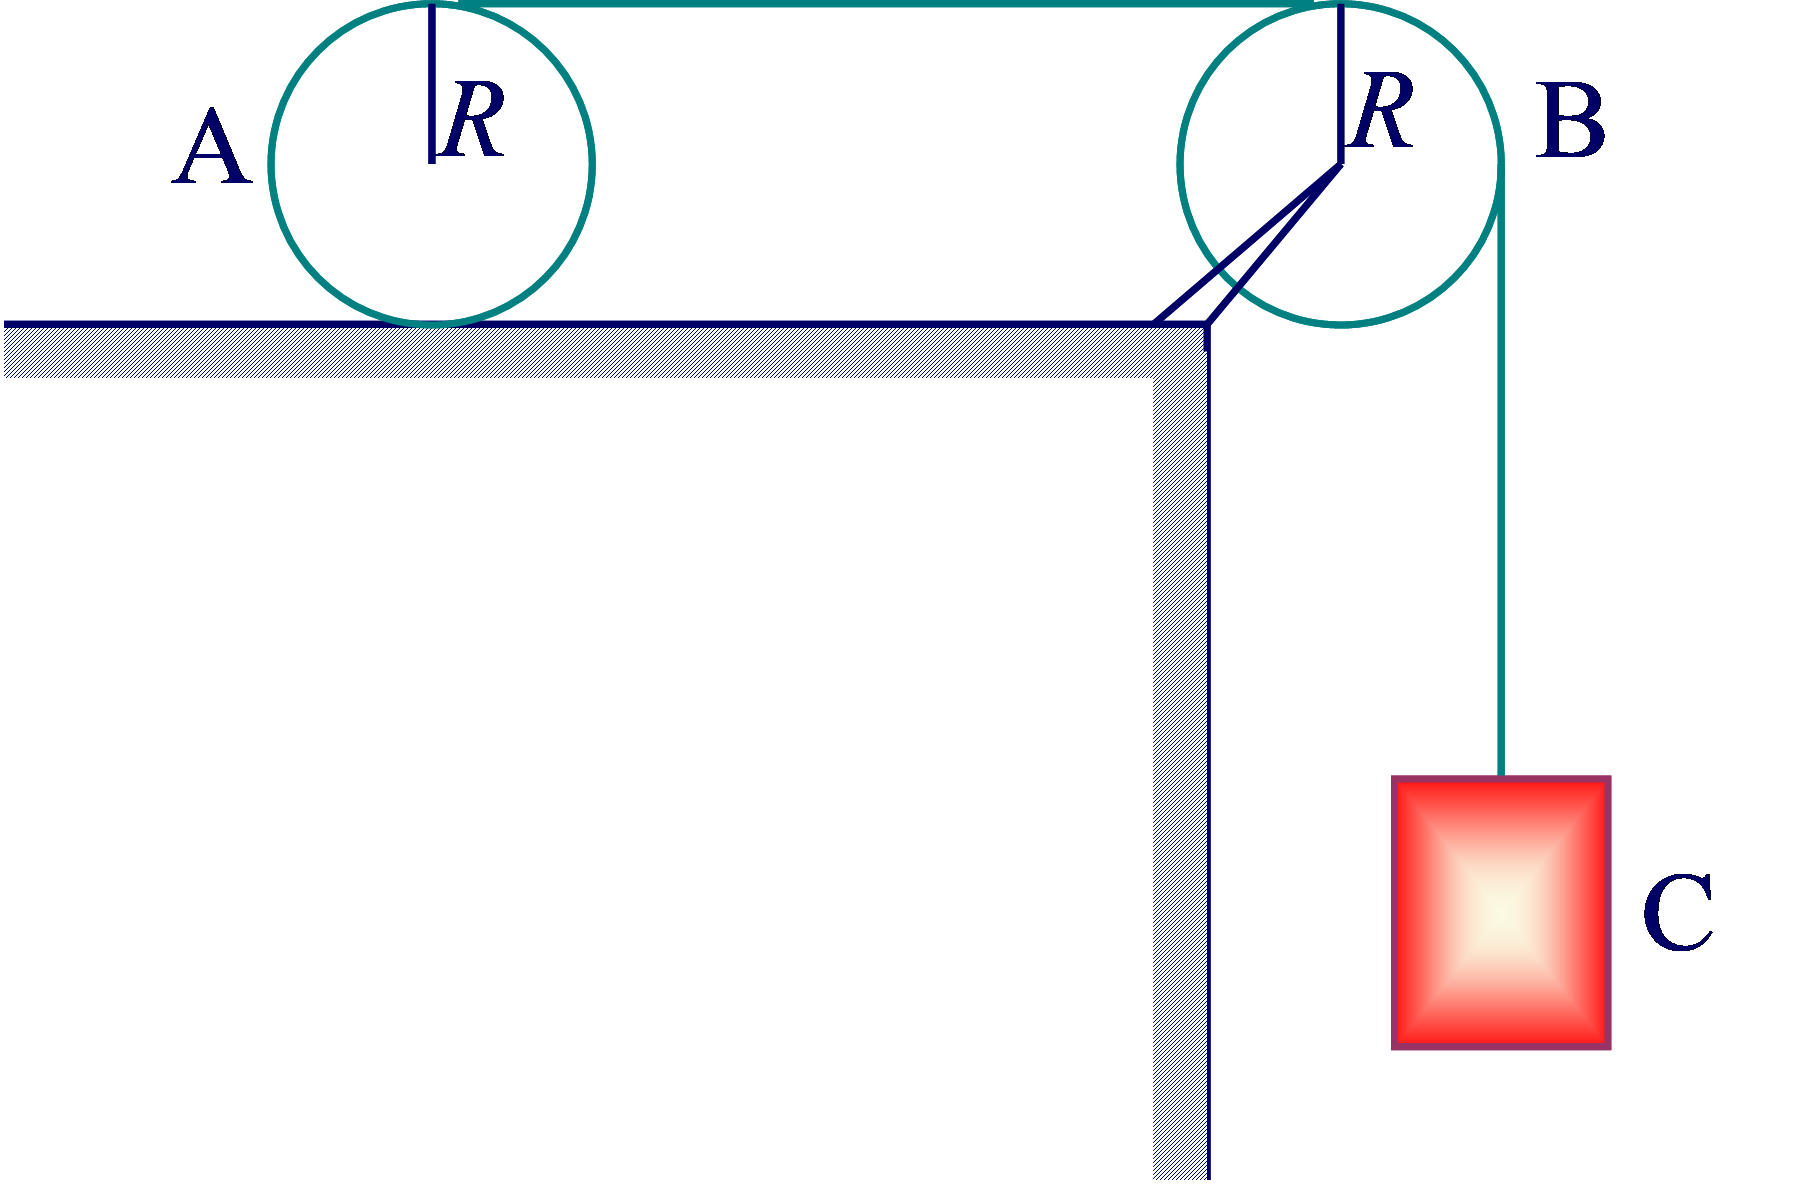
\includegraphics[width=5cm,height=4cm,keepaspectratio]{figures/image9.png}\par}\medskip

（1）圆柱体 A 与桌面间的摩擦力;

（2）物体 C 下落 h 后的速度和加速度大小。

\pdfbookmark[1]{四．(16分) 如图所示，已知弹簧的劲度系数为k，物体的质量为m，滑轮的半径为R，质量为M。开始时托住物体m，使得系统保}{section11}

四．(16 分) 如图所示，已知弹簧的劲度系数为 k，物体的质量为 m，滑轮的半径为 R，质量为 M。开始时托住物体 m，使得系统保持静止，绳子刚好拉直而弹簧无形变，t=0 时放开 m。设绳子与滑轮间无相对滑动，滑轮可视为均质圆盘。\par\medskip{\centering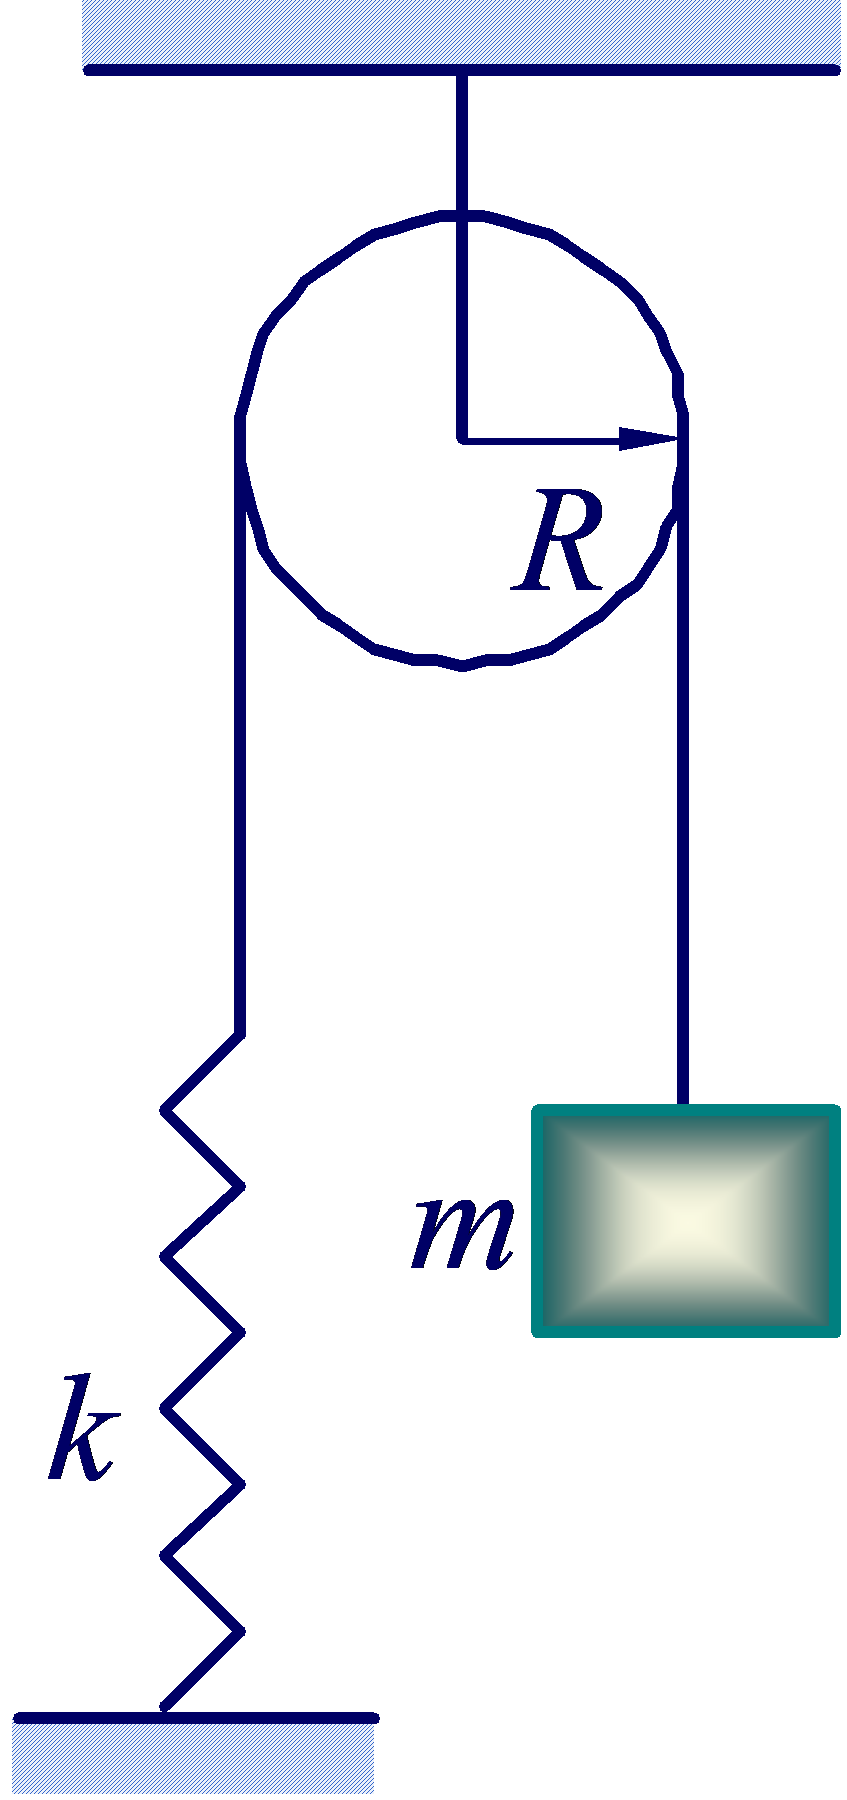
\includegraphics[width=5cm,height=4cm,keepaspectratio]{figures/image10.png}\par}\medskip

(1)放开后 m 是否作简谐振动？若是，试求出振动周期 T；

(2)写出 m 的振动表达式。

\pdfbookmark[1]{五．如图所示，一沿X轴正方向传播的平面简谐波从波疏媒质垂直入射到波密媒质上的B点并发生反射后形成的逆X轴传播的反射波（振}{section14}

五．如图所示，一沿 X 轴正方向传播的平面简谐波从波疏媒质垂直入射到波密媒质上的 B 点并发生反射后形成的逆 X 轴传播的反射波（振幅无衰减）。已知波源位于坐标原点 O 处，O 点到反射点 B 的距离 L=10 m，入射波的振幅\(A = 0.2\)(m)，频率\(\nu = 2\)(Hz)，波长λ=6m，当 t=0 时，波源离开平衡位置\(\sqrt{2}A/2\)，且向负 Y 方向运动，求 (1)入射波方程；(2)反射波方程；(3)OB 间因入射波和反射波干涉而静止的点的位置.\par\medskip{\centering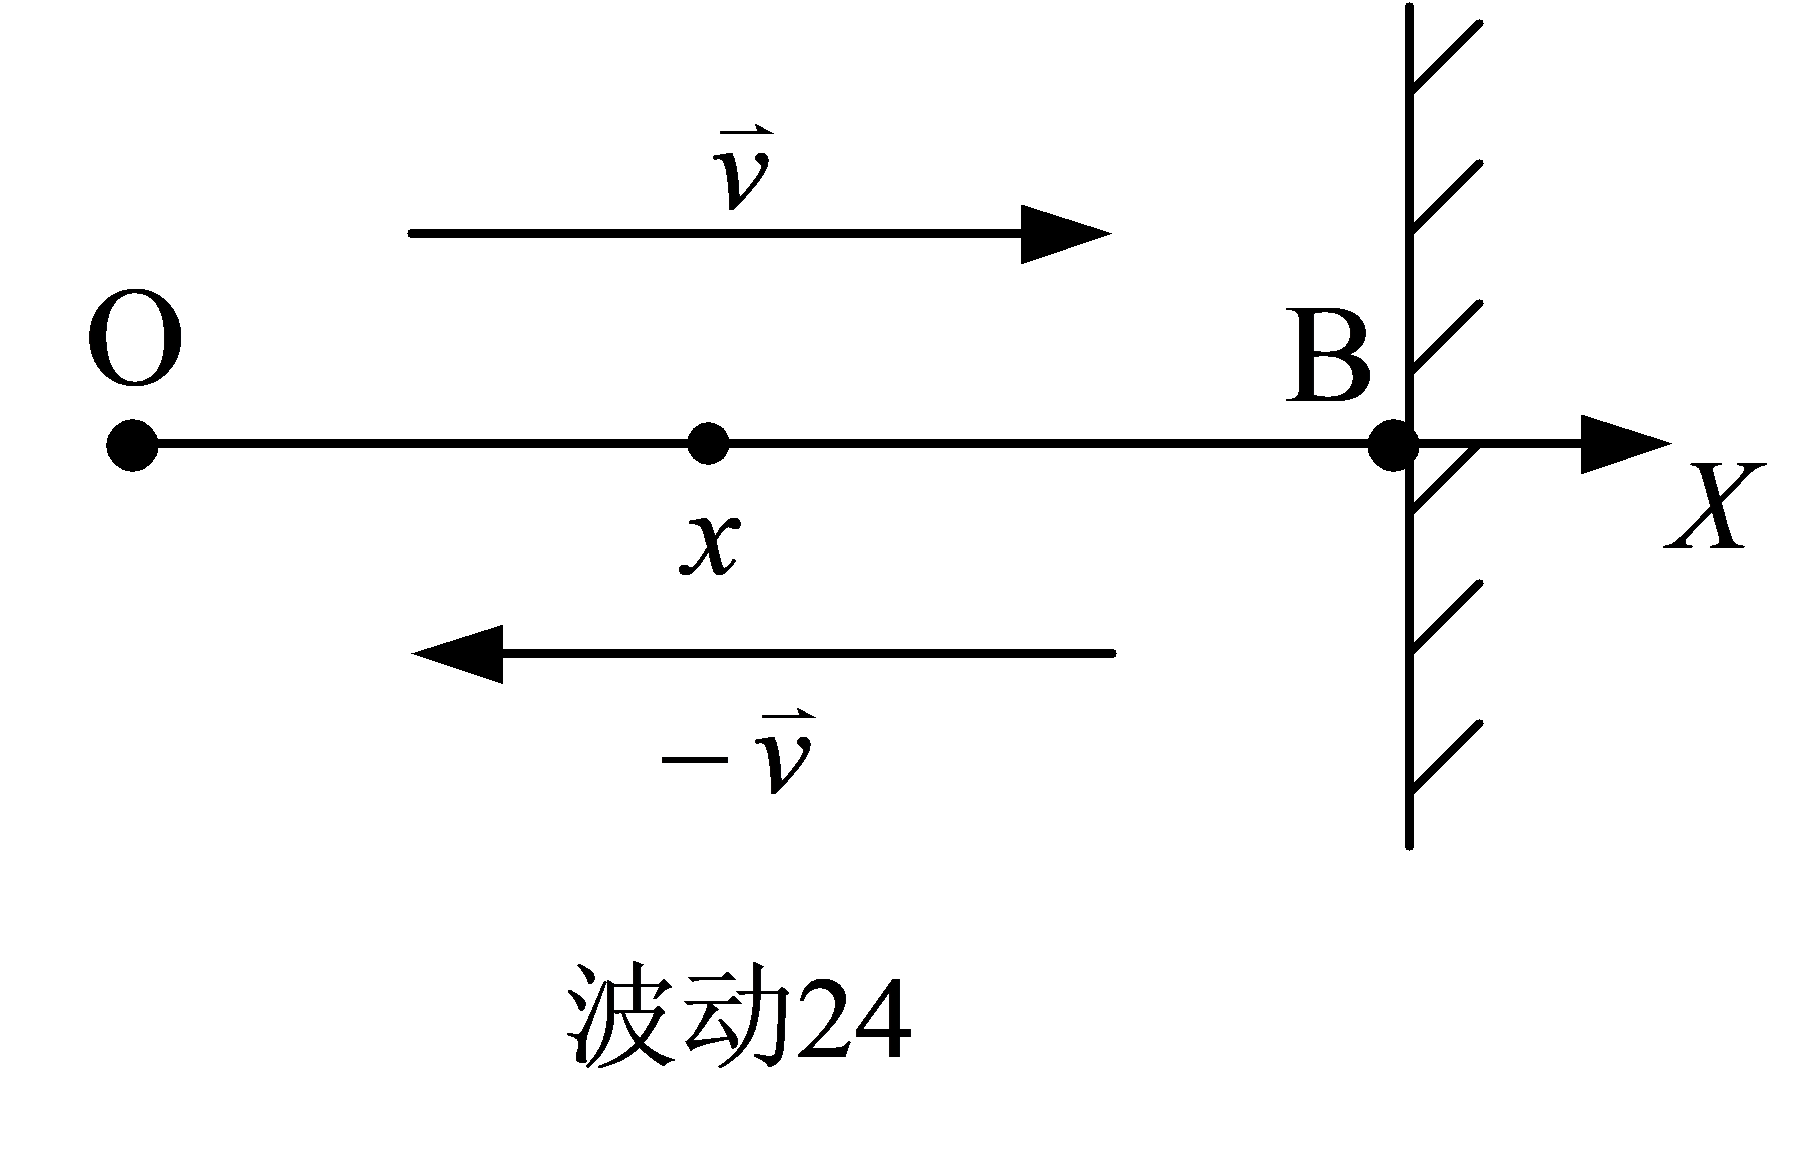
\includegraphics[width=5cm,height=4cm,keepaspectratio]{figures/image11.png}\par}\medskip

\pdfbookmark[1]{六. (16分) 一宇宙飞船A以0.8c的速度平行于地面飞行。宇宙飞船上的宇航员测得此飞船的长度为60米。问：}{section15}

六. (16 分) 一宇宙飞船 A 以 0.8c 的速度平行于地面飞行。宇宙飞船上的宇航员测得此飞船的长度为 60 米。问：

（1）地面上的观测者测得的飞船 A 的长度为多少？

（2）若有另一飞船 B 相对地面以 0.8c 的速度沿相反方向飞行，问 A 飞船上的观测者所测得的 B 飞船的速度大小。

\end{document}
